%\documentclass[handout]{beamer}

\documentclass[pdf]{beamer}
\usetheme{Warsaw}
%List of themes{Warsav Malmoe Antibes Boadilla Frankfurt Juanlespins Montpellier Singapore Bergen Copenhagen Goettingen Madrid Paloalto Berkeley Darmstadt Hannover Malmoe Pittsburgh Berlin Dresden Ilmenau Marburg Rochester}
%\usecolortheme{seagull}
%List of colours{albatross	crane	beetle	dove fly	seagull wolverine beaver}
\usepackage{beamerthemesplit}
\usepackage{graphicx}
\usepackage{epstopdf}
\usepackage{latexsym}
\usepackage{amsmath}
\usepackage{ulem}
%\xdefinecolor{lavendar}{rgb}{0.8, 0.6, 1}http://www.software995.com/
%\setbeamercolor{frametitle}{fg=black, bg=lavendar}
\usepackage{verbatim}
\usepackage{hyperref}
\usepackage{helvet}



\title{Moment Inequalities\thanks{%
These notes are adapted from Ariel Pakes' lecture notes from previous years'
graduate classes at Harvard, and from Kate Ho's subsequent adaptations.}}
\author{Julie Holland Mortimer}
\date{Economics 853}

%%%%%%%%%%%%%%%%%%%%%%%%%%%%%%%%%%%%%%%%%%%%%%%%%%
%%%%%%%%%%%%%%%%%%%%%%%%%%%%%%%%%%%%%%%%%%%%%%%%%%%

\begin{document}
% outline at the beginning of each section
%\AtBeginSection[]
%{
%\begin{frame}[plain]
% \frametitle{Outline}
% \tableofcontents[currentsection] 
% \normalsize
%\end{frame}
%}

\frame[plain]{\titlepage}

\section[Outline]{}
\frame[plain]{
\frametitle{Outline}
\tableofcontents}

\section{Overview}

\frame[plain]
{
\frametitle{Overview}
In this lecture we explore recent approaches to estimating models through the use of inequality restrictions, rather than equality restrictions.  \\
\vspace{0.2in}
The motivation for these approaches comes from:

\begin{itemize}
\item Economic problems that cannot be empirically investigated with
more standard techniques (e.g., discrete games)

\item Sampling methodology or measurement limitations in data (e.g. we don't know an agent's exact income, but we know whether it lies in an
interval, so we can get inequalities on income; or
we have topcoded income)
\end{itemize}
}

\frame[plain]
{
The assumptions required in the latter case to ensure that moment
inequalities estimators have desirable properties are quite straightforward.\\
\vspace{0.2in}
The assumptions required in the former case are more subtle. \\
\vspace{0.2in}
Once we investigate these assumptions, we may start questioning the assumptions underlying the estimators of more traditional behavioral problems (particularly those that
require discrete actions in a game). 

\frametitle{Overview}
}

\frame[plain]
{
\frametitle{Overview}
The appeal of using moment inequalities to analyze a behavioral model is
that the set up for the econometric problem is often the same as the set up for a
theoretical model. \\
\vspace{0.2in}
This similarity makes it easy to interpret the results in a way that
is consistent with the theory. \\
\vspace{0.2in}
However, dealing with unobservables can be tricky in this context. 


}
\section{Economic Model}
\frame[plain]
{
\frametitle{Economic Model}

\begin{itemize}
\item The econometrician observes a set of choices made by various agents.
\vspace{0.1in}

\item Assume agents expect the choices they made to lead to returns that are
higher than the returns they would have earned had they made an
alternative feasible choice.
\vspace{0.1in}

\item Assume a parametric ``return function.'' 
\vspace{0.1in}

\item For each value of $\theta $, compute the difference between the observable part of the actual realized returns and the observable part of returns the agents would have earned had they made the alternative choice.
\end{itemize}
}

\frame[plain]
{
\frametitle{Economic Model}
\begin{itemize}

\item Estimator:\ Accept any value of $\theta $ that, on average, makes the
observed decisions better (more profitable)\ than the alternative.
\vspace{0.1in}

\item Question:\ When do such (possibly set valued) estimators enable us to
make valid inferences on the parameters of interest?
\end{itemize}

}

\frame[plain]
{
\frametitle{Economic Model}

There is more than one set of conditions that can be used to justify
inequality estimators.  We will consider the following two such sets of conditions:\\
\begin{itemize}
\vspace{0.1in}
\item The set that uses only ``structural errors'' (i.e., assumptions
that are the multiple-agent analog of the assumptions used in discrete
choice econometrics). \\
\vspace{0.1in}

\item The set that incorporates expectational and measurement errors along with the structural errors.\\


\end{itemize}
}

\frame[plain]
{
\frametitle{Economic Model}
\begin{itemize}
\item  Ciliberto and Tamer \textit{(Econometrica 2009)} develop the estimator based on the first set of conditions in the context of an entry model.\\
\vspace{0.1in}
\item Pakes, Porter, Ho and Ishii \textit{(Econometrica 2015)} develop the estimator based on the second set of conditions.\\
\vspace{0.1in}
\item  Pakes\ \textit{(Econometrica 2010)} provides a comparison of the two sets of conditions.\\
\end{itemize}
}




\section{Conditions Common to the Two Inequality Estimators}


\frame[plain]
{
\frametitle{Conditions Common to the Two Inequality Estimators}
Recall the first two conditions that are relevant to discrete games.  We covered these in the last lecture.\\

\begin{enumerate}
\item \textbf{Nash Condition\ (C1)}
\begin{equation*}
\sup_{d\in D_{i},d\neq d_{i}}\mathit{\varepsilon }\left[ \pi (d,\mathbf{d}_{-i},%
\mathbf{y}_{i},\theta _{0})|\mathit{I}_{i}\right] \leq \mathit{\varepsilon }%
\left[ \pi (d_{i},\mathbf{d}_{-i},\mathbf{y}_{i},\theta _{0})|\mathit{I}_{i}%
\right] 
\end{equation*}
where $D_{i}\subset D$, for $i=1,...,n$.\\
\vspace{0.1in}
\item \textbf{Counterfactual Condition\ (C2)}

\begin{equation*}
\mathbf{d}_{-i}=d^{-i}(\mathbf{d}_{i},\mathbf{z}_{i}),\text{ \ }\mathbf{y}%
_{i}=y(\mathbf{z}_{i},\mathbf{d}_{i},\mathbf{d}_{-i}),\text{ }and
\end{equation*}
the distribution of $\mathbf{z}_{i}$ conditional on $\mathit{I}_{i}$ does
not depend on $d_{i}$.

\end{enumerate}
}
\frame[plain]
{\textbf{Implications of conditions C1 and C2:}\\
\vspace{0.2in}
If $d^{\prime }\in D_{i}$ and 
\begin{equation*}
\Delta \pi (d_{i},d^{\prime },d_{-i},z_{i})=\pi (d_{i},d_{-i},z_{i})-\pi
(d^{\prime },d_{-i},z_{i})
\end{equation*}
then%
\begin{equation*}
\mathit{\varepsilon }\left[ \Delta \pi (d_{i},d^{\prime },\mathbf{d}_{-i},%
\mathbf{z}_{i})|\mathit{I}_{i}\right] \geq 0.
\end{equation*}

To use this inequality directly as a basis for an estimation algorithm, we need the
relationships between:

\begin{itemize}
\item The expectations underlying agents' decisions ($\mathit{\varepsilon }(.)$%
) and the expectations of the observed sample moments ($E(.)$),

\item $\pi (.,\theta )$ and $(z\,_{i},d_{i},d_{-i})$ and their observable
analogues.
\end{itemize}

This is where the two approaches differ.  We covered the first set in the last lecture.
\frametitle{Conditions Common to the Two Inequality Estimators}
}
\section{Extra Conditions under Full\ Information and No
Specification Error}
\frame[plain]
{
\frametitle{Extra Conditions under Full\ Information and No
Specification Error}
\begin{enumerate}
\setcounter{enumi}{2}
  \item \textbf{ Expectational Condition (FC3)}
\begin{equation*}
\pi (d,d_{-i},z_{i},\theta _{0})=\mathit{\varepsilon }\left[ \pi (d,\mathbf{d}%
_{-i},\mathbf{z}_{i},\theta _{0})|\mathit{I}_{i}\right] 
\end{equation*}
\begin{equation*}
\forall d\in D_{i}.
\end{equation*}

\item \textbf{Measurement Conditions (FC4)}

\begin{equation*}
\pi (.,\theta )\text{ is known.}
\end{equation*}%
\begin{equation*}
z_{i}=(\upsilon _{2,i}^{f},z_{i}^{o})\text{ },\text{ }%
(d_{i},d_{-i},z_{i}^{o},z_{-i}^{o})\text{ observed,}
\end{equation*}%
\begin{equation*}
(\upsilon _{2,i}^{f},\upsilon _{2,-i}^{f})|_{z_{i}^{o},z_{-i}^{o}}\sim
F(.;\theta )\text{, }F(.,\theta )\text{ is known.}
\end{equation*}

\end{enumerate}
}

\frame[plain]
{
\frametitle{Extra Conditions under Full Information and No
Specification Error}
\textbf{Implications of conditions FC3 and FC4:}\\
\begin{equation*}
\Delta \pi (d_{i},d^{\prime },d_{-i},z_{i}^{o},\upsilon _{2,i}^{f};\theta
_{0})\geq 0,
\end{equation*}
\begin{equation*}
\forall d\in D_{i}\mbox{, and}
\end{equation*}
\begin{equation*}
(\upsilon _{2,i}^{f},\upsilon _{2,-i}^{f})|_{z_{i}^{o},z_{-i}^{o}}\sim
F(.;\theta _{0}).
\end{equation*}
(Note that there may not be a $\theta $ that satisfies these
conditions for all vectors of decisions.) To ensure that the model assigns
positive probability to the observed decisions for some $\theta $ we
typically also assume:%
\begin{equation*}
\pi (d_{i},d_{-i},z_{i}^{o},\upsilon _{2,i}^{f})=\pi
^{as}(d,d_{-i},z_{i}^{o},\theta _{0})+\upsilon _{2,i,d}^{f},
\end{equation*}
and that the distribution $\upsilon _{2,i}^{f}$ conditional on $\upsilon
_{2,-i}^{f}$ has full support.
}

\section{Estimation from Inequality Conditions (Structural Errors Only)}

\frame[plain]
{
\frametitle{Estimation from Inequality Conditions (Structural Errors Only)}
This section follows Ciliberto and Tamer (2009), which studies entry in the airline industry.\\
\vspace{0.1in}
Start with the  formulation of profit in Berry (1992):

\begin{equation*}
\Pi_{m,k,N} =X_{m} \beta - \delta \text{log} N + Z_k \alpha +  (\rho u_{m0} + \sqrt{1- \rho^2} u_{mk})
\end{equation*}

\begin{itemize}
\item $(X_{m} \beta - \delta \text{log} N) $ is the observable component of profit that is common to all firms in a market
\item $Z_k \alpha$ is the observable component of profit that varies across firms within a market. 
\item The unobserved components of profit also have a common component $(\rho u_{m0}) $ and a firm-specific component ($\sqrt{1- \rho^2} u_{mk}$).
\end{itemize}

}

\frame[plain]
{
\frametitle{Estimation from Inequality Conditions (Structural Errors Only)}
Ciliberto and Tamer allow for a more flexible profit function, seen here:

\begin{equation*}
\Pi_{m,i} =S_m'\alpha + Z_{im}' \beta_i + W_{im}'\gamma_i + \sum_{j \neq i} \delta_{j}^{i}y_{jm} + \sum_{j \neq i} Z_{jm}'\phi_j^i y_{jm} + \epsilon_{im}
\end{equation*}

\noindent
\footnotesize
Definitions: \\
$S_m$ denotes market characteristics common to all firms\\
$Z_{im}$ is a vector of firm characteristics that enter into the profits of all firms in the market (e.g., product attributes that consumers value)\\
$W_{im}$ is a vector of firm characteristics that only affect firm $i$'s profit in market $m$\\
$y_{jm}$ is an indicator for the presence of other firms $j\neq i$ in market $m$\\
$\delta_{j}^{i}$ captures the effect of having firm $j$ in market $m$ on firm $i$'s profit\\
$\phi_j^i$ captures firm-interaction effects that arise through the $Z_m$'s.\\
$\epsilon_{im}$ has several components: destination, origin, airport, and a firm-market unobservable.  This maps to the $\upsilon_{2,i}$ error in our notes, and is assumed to be observed by all players.\\
%$K$ is the number of potential entrants in market $m$\\

}

\frame[plain]
{
\frametitle{Estimation from Inequality Conditions (Structural Errors Only)}
We can write down the conditions from the theoretical model (C1 and C2) given this profit function, as well as the conditions that allow us to translate the theoretical model to the data in a perfect information, ``structural errors'' world (FC3 and FC4).  \\
\vspace{0.2in} 
Note that although the model
does specify a parametric distribution for the $(\upsilon
_{2,i}^{f},\upsilon _{2,-i}^{f})$ conditional on the observables, it does
not deliver a likelihood.  \\
\vspace{0.2in} There is no function that takes values of the $%
z^{o},\upsilon _{2}$ and $\theta $ vectors into uniquely-specified actions,
so we cannot construct probabilities for those actions.  \\
\vspace{0.2in} 
This result comes directly from the inequalities of the entry game, and is due to the possibility of multiple equilibria.  
}

\frame[plain]
{
\frametitle{Results/Conditions that the Inequalities \\with FC3 and FC4 Deliver}

\begin{enumerate}
\item We can check whether the conditions of the model are satisfied at the
observed $(d_{i},d_{-i})$ for any $(\upsilon _{2,i}^{f},\upsilon
_{2,-i}^{f}) $ and $\theta $, and this, together with $F(.,\theta )$,
enables us to calculate the probability of those conditions being satisfied
at any $\theta $. \\
\vspace{0.2 in} 
These are necessary conditions for the choice to be made:\
therefore when $\theta =\theta _{0}$ the probability of satisfying them must
be weakly greater than the probability of observing $(d_{i},d_{-i})$. \\
\vspace{0.2 in} 
I.e. the model delivers an \textit{outer measure}\ for the actions conditional on $%
\theta $.
\end{enumerate}
}

\frame[plain]
{
\frametitle{Results/Conditions that the Inequalities \\with FC3 and FC4 Deliver}
\begin{enumerate}
\setcounter{enumi}{1}
\item We can check whether $(d_{i},d_{-i})$ are the only values of the
decision variables to satisfy the necessary conditions for any $(\upsilon
_{2,i}^{f},\upsilon _{2,-i}^{f})$ and $\theta $, and this can be used to
provide a lower bound on the probability of actually observing $%
(d_{i},d_{-i})$ given $\theta $. \\
\vspace{0.2in}
When $\theta =\theta _{0}$ the probability
that we observe these decisions is weakly greater than the probability that
they're the only values that are consistent with the model. \\
\vspace{0.2 in} 
I.e., the model also delivers an \textit{inner measure} for the action conditional on $\theta $.
\end{enumerate}

}

\frame[plain]
{
\frametitle{Results/Conditions that the Inequalities \\with FC3 and FC4 Deliver}
More formally, define the probability that the model generated by C1, C2,
FC3 and FC4 with the additive separability constraint, a model we will call
MF, is satisfied at a particular $(d_{i},d_{-i})$ for a given $\theta $ to
be: 
\begin{equation*}
\bar{P}\left\{ (d_{i},d_{-i})|\theta \right\} =\Pr \left\{ (\upsilon
_{2,i}^{f},\upsilon _{2,-i}^{f}):(d_{i},d_{-i})\text{ satisfy MF}%
|z_{i}^{o},z_{-i}^{o},\theta \right\} ,
\end{equation*}%
and the analogous lower bound to be:%
\begin{equation*}
\text{\b{P}}\left\{ (d_{i},d_{-i})|\theta \right\} =\Pr \left\{ (\upsilon
_{2,i}^{f},\upsilon _{2,-i}^{f}):\text{only }(d_{i},d_{-i})\text{ satisfy MF}%
|z_{i}^{o},z_{-i}^{o},\theta \right\} .
\end{equation*}
}

\frame[plain]
{
\frametitle{Results/Conditions that the Inequalities \\with FC3 and FC4 Deliver}
Were we to know the equilibrium selection mechanism we could also calculate
the actual likelihood of $(d_{i},d_{-i})$ for a given $\theta $ or%
\begin{equation*}
P\left\{ (d_{i},d_{-i})|\theta \right\} =\Pr \left\{
(d_{i},d_{-i})|z_{i}^{o},z_{-i}^{o},\theta \right\} .
\end{equation*}

We \textit{do not know} the selection mechanism but we do know that for the true
selection mechanism when $\theta =\theta _{0}$%
\begin{equation*}
\boxed{\bar{P}\left\{ (d_{i},d_{-i})|\theta \right\} \geq P\left\{
(d_{i},d_{-i})|\theta \right\} \geq \text{\b{P}}\left\{
(d_{i},d_{-i})|\theta \right\} .}
\end{equation*}
}

\frame[plain]
{
\frametitle{Results/Conditions that the Inequalities \\with FC3 and FC4 Deliver}
Let $\left\{ {}\right\}$ be the indicator function which takes the value
one if the condition inside the brackets is satisfied and zero elsewhere.\\
\vspace{0.2in}
Let $h(.)$ be a function which takes only positive values.\\
\vspace{0.2in}
Let $E(.)$ provide expectations conditional on the process actually generating the data
(including the equilibrium selection process).
}

\frame[plain]
{
\frametitle{Results/Conditions that the Inequalities \\with FC3 and FC4 Deliver}
 Then\ MF implies that%
\begin{equation*}
E_{\upsilon _{2}}(N^{-1}\sum_{i}(\bar{P}\left\{ (d_{i},d_{-i})|\theta
\right\} -\left\{ d=d_{i},d^{-i}=d_{-i}\right\} )h(z_{i}^{o},z_{-i}^{o}))
\end{equation*}%
\begin{equation*}
=\boxed{N^{-1}\sum_{i}(\bar{P}\left\{ (d_{i},d_{-i})|\theta \right\} -P\left\{
(d_{i},d_{-i})|\theta \right\} )h(z_{i}^{o},z_{-i}^{o})\geq 0\text{ }at\text{
}\theta =\theta _{0}\text{.}}
\end{equation*}

which gives us a moment inequality. An analogous moment inequality can be
constructed from the condition on \b{P}$\left\{ (d_{i},d_{-i})|\theta
\right\}$:

\begin{equation*}
=\boxed{N^{-1}\sum_{i}(P\left\{(d_{i},d_{-i})|\theta \right\} - \b{P}\left\{ (d_{i},d_{-i})|\theta \right\})
h(z_{i}^{o},z_{-i}^{o})\geq 0\text{ }at\text{
}\theta =\theta _{0}\text{.}}
\end{equation*}

}


\frame[plain]
{
\frametitle{Estimation Routine - Ciliberto and Tamer (2009)}
The estimation routine:
\begin{itemize}
\item constructs unbiased estimates of $(\b{P}(\cdot|\theta),\bar{P}(\cdot|\theta))$, 
\item substitutes them for the true values of the probability bounds into these moments, and
\item accepts values of  $\theta$ for which the moment inequalities are satisfied.
\end{itemize}
\vspace{0.1in}
Since typically neither the upper nor the lower bound are
analytic functions of $\theta$, we employ simulation techniques to obtain an unbiased estimate of them.\\
\vspace{0.2in}
%%%%%%%%%Julie - we cut out the following detail on the simulation techniques
%The simulation procedure is straightforward, though often computationally burdensome.
}
%
%\frame[plain]
%{
%\frametitle{Estimation Routine - Ciliberto and Tamer (2009)}
%Take pseudo random draws from a standardized version of $F(\cdot)$
%as defined in FC4, and for each random draw check the necessary 
%conditions for an equilibrium, at the observed $(d_i, d_{-i})$.\\
%\vspace{0.2in}
%Estimate $\bar{P}(d_i, d_{-i}|\theta)$ by the fraction of random draws that satisfy 
%that inequality at that $\theta$. Next check if there is another
%value of $(d_i, d_{-i}) \in D_i \times D_{-i}$ that satisfies the equilibrium conditions at that 
%$\theta$ and estimate $\b{P}(d_i, d_{-i}|\theta)$ by the fraction of the
%draws for which $(d_i, d_{-i})$ is the only such value.
%
%}
%
%\frame[plain]
%{
%\frametitle{Estimation Routine - Ciliberto and Tamer (2009)}
%If there are $ns$ simulation draws for each market $j$ with number 
%of actors $n(j)$ and cardinality of the choice set $O(D(j))$, then:
%\begin{itemize}
%\item to construct $\bar{P}( \cdot | \theta))$ we need to check $ns \times \sum O( D(j))$ for %each market, and
%\item to construct $\b{P}( \cdot | \theta)$ we need $ns \times \sum O(D(j))^{n(j)}$ equilibrium
%conditions for each $\theta$ evaluated in the estimation routine. \\
%\vspace{0.2in}
%\end{itemize}
%If this were a two-period structural model (rather than a reduced-form
%for profit), then typically every evaluation would require an
%evaluation of the second stage profit function. 
%}
%%%%%%%%%%%%%%%%%%%%%%%End Cut Section
\frame[plain]
{
\frametitle{Estimation Routine - Ciliberto and Tamer (2009)}This process can be computationally expensive, often too computationally burdensome
to do. \\
\vspace{0.2in}
We can get away with fewer function evaluations if
we want to rely only on the upper bound probability $\bar{P}( \cdot | \theta))$, as
then we can drop as many comparisons as we want, though by
dropping inequalities you are likely to widen the set of  $\theta$ the
model accepts.
}

\frame[plain]
{
\frametitle{Data - Ciliberto and Tamer (2009)}
The same data used in Berry (1992):
\begin{itemize}
\item DB1B data from 2001 (no price data).  
\item A market is a trip between two airports and a direction, regardless of stops. 
\item The data covers a sample of markets between the top 100 MSA's; 2742 markets.   \item Ciliberto and Tamer focus on strategic interactions between American, Delta, United, and Southwest and pay particular attention to Dallas because of the Wright Amendment.  
\item They construct Berry's ``airport presence'' variable; they do not have cost data, but they have plane capacities and they use that to construct an opportunity fixed cost of serving a market.
\end{itemize}
}

\frame[plain]
{
\frametitle{Results - Ciliberto and Tamer (2009)}
Tables 3 and 4 in Ciliberto and Tamer report confidence intervals for points (i.e. the probability that the confidence set covers the identified set is .95). Table 3 assumes iid errors.  \\

\vspace{0.1in}
\begin{itemize}
\item The first column constrains competitive effects of each firm's presence in the market on other firms to be the
same.  So, as in Berry (1992) there is a unique number of
firms. The competitive effects (number of other airlines 
serving the city-pair) and the airport presence effect are
both strong, as in prior work.
\end{itemize}
}

\frame[plain]
{
\frametitle{Results - Ciliberto and Tamer (2009)}
\begin{itemize}
\item Column 2 allows competitive effects to vary across firms. No longer
a unique number of firms (depends on who enters). Competitive effects 
are similar except for the low-cost carriers
which have a bigger impact, and airport presence stronger yet.\\
\vspace{0.2in}
\item Column 4 allows one airline's presence to affect different airlines differently. Now Large airlines (LAR) and Southwest (=WN) have strongly negative effects on LCC, and there
are smaller differences among the rest.
\end{itemize}

}

\frame[plain]
{
\frametitle{Results - Ciliberto and Tamer (2009)}
\begin{center}
\hspace{-.43in}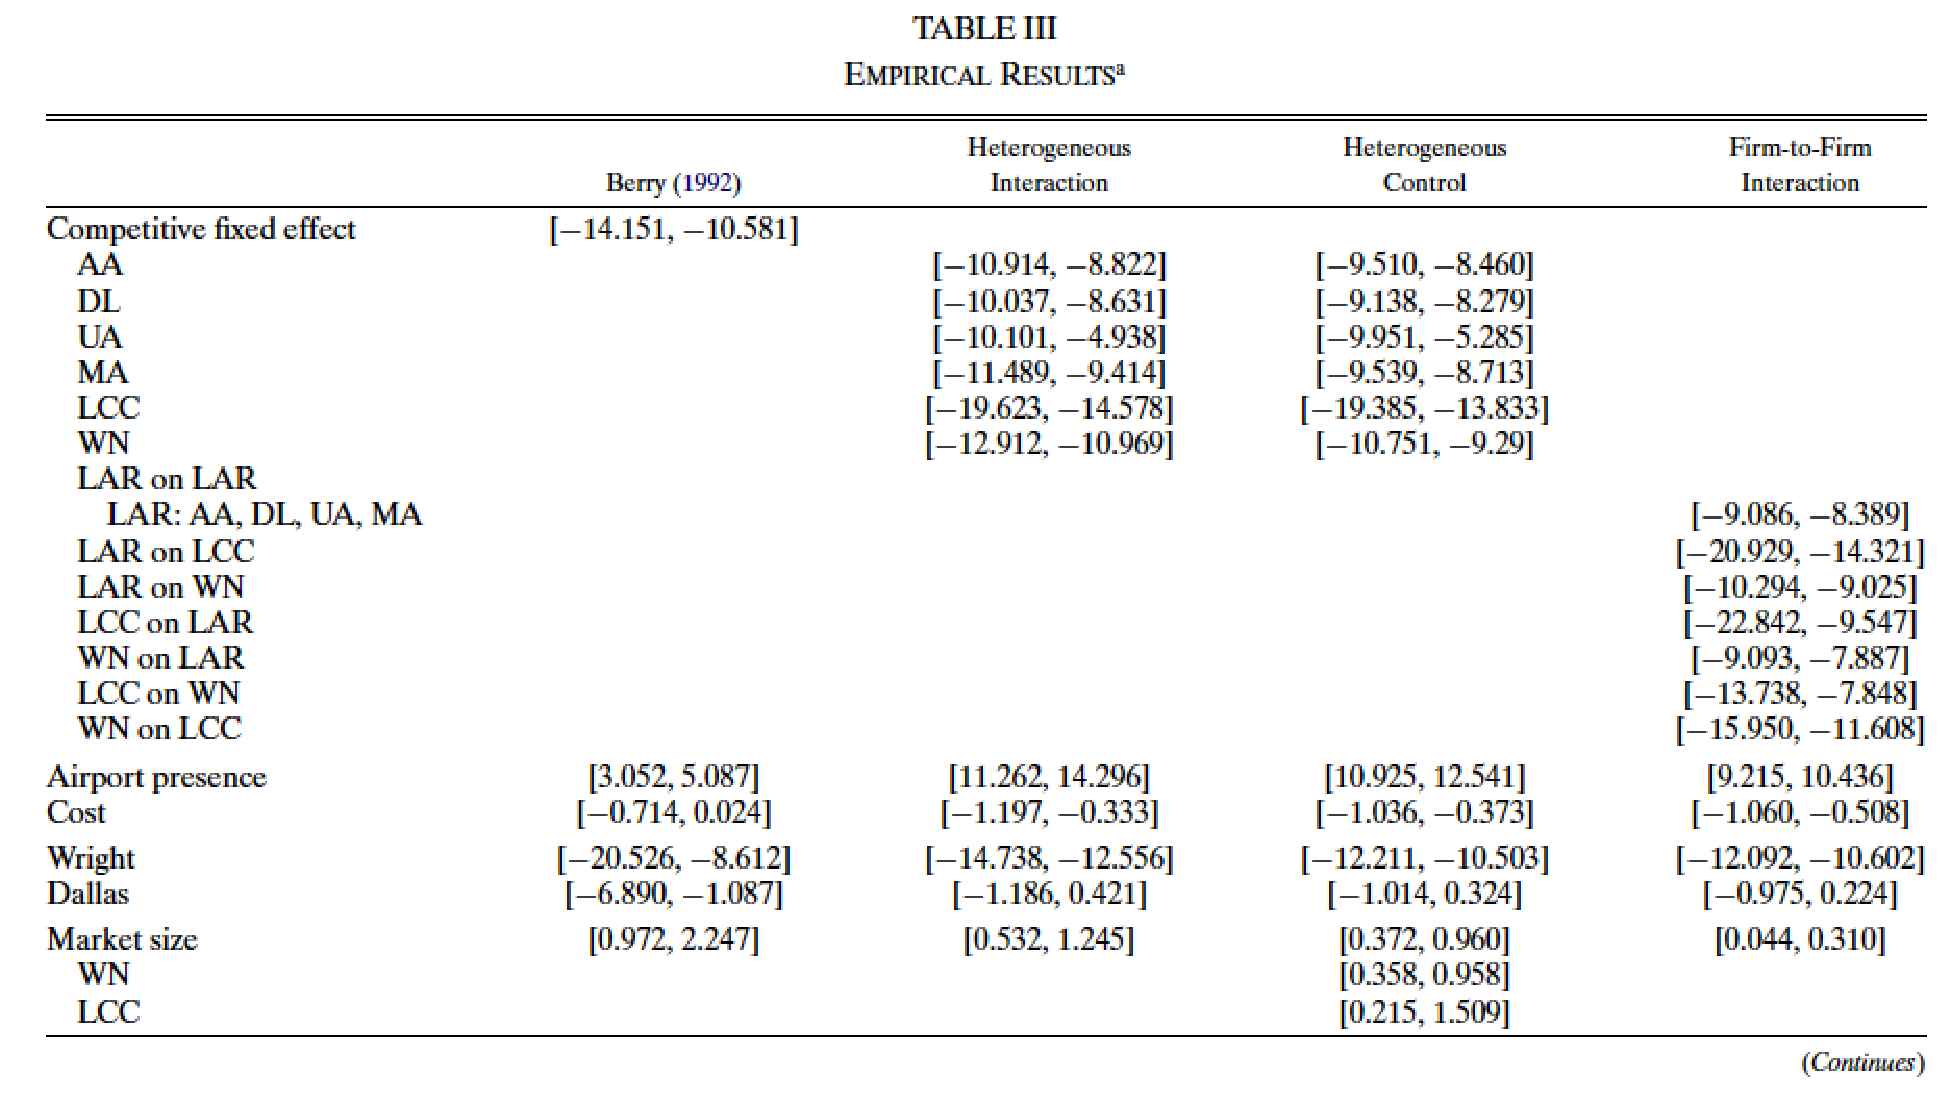
\includegraphics[width=1.1\linewidth]{ciliberto_tamer_table3a.pdf}\\
\end{center}
}

\frame[plain]
{
\frametitle{Results - Ciliberto and Tamer (2009)}
\begin{center}
\hspace{-.43in}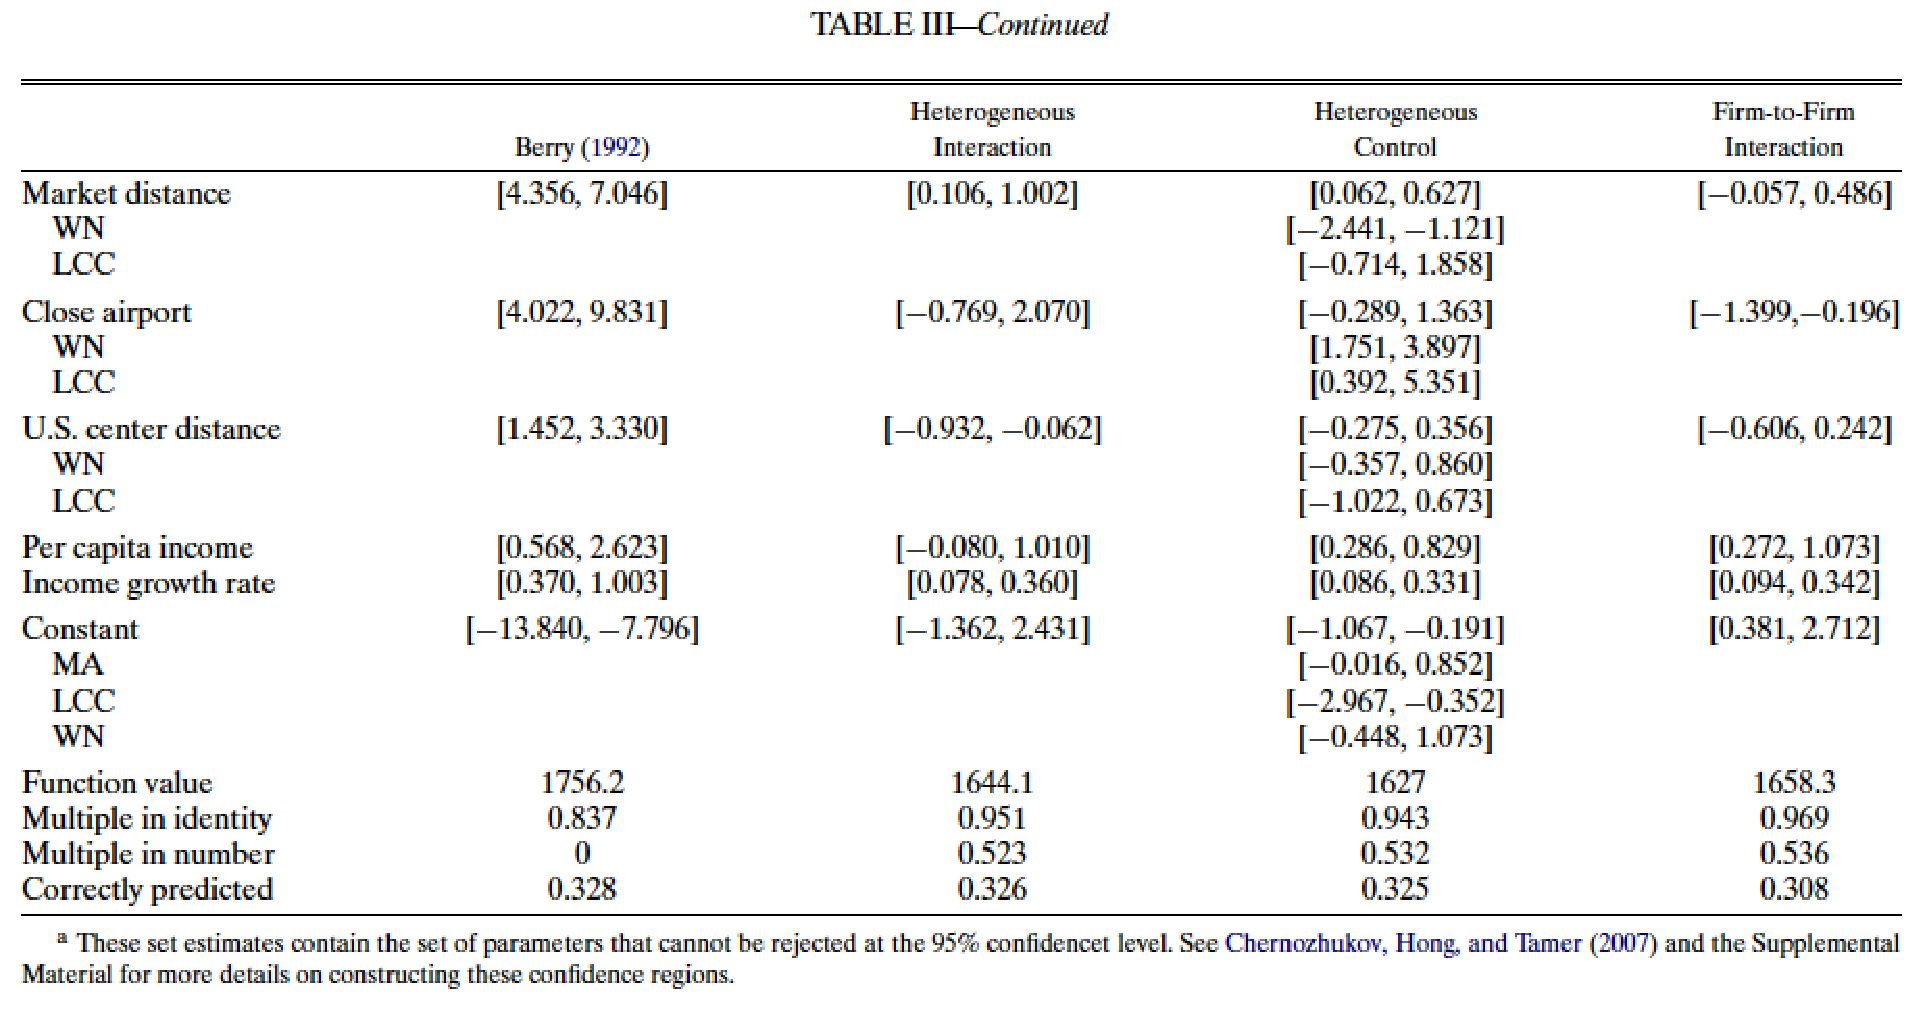
\includegraphics[width=1.1\linewidth]{ciliberto_tamer_table3b.pdf}\\
\end{center}
}


\frame[plain]
{
\frametitle{Results - Ciliberto and Tamer (2009)}
\begin{center}
\tiny
TABLE IV\\
{\sc Variable Competitive Effects}\\
\hspace{-.43in}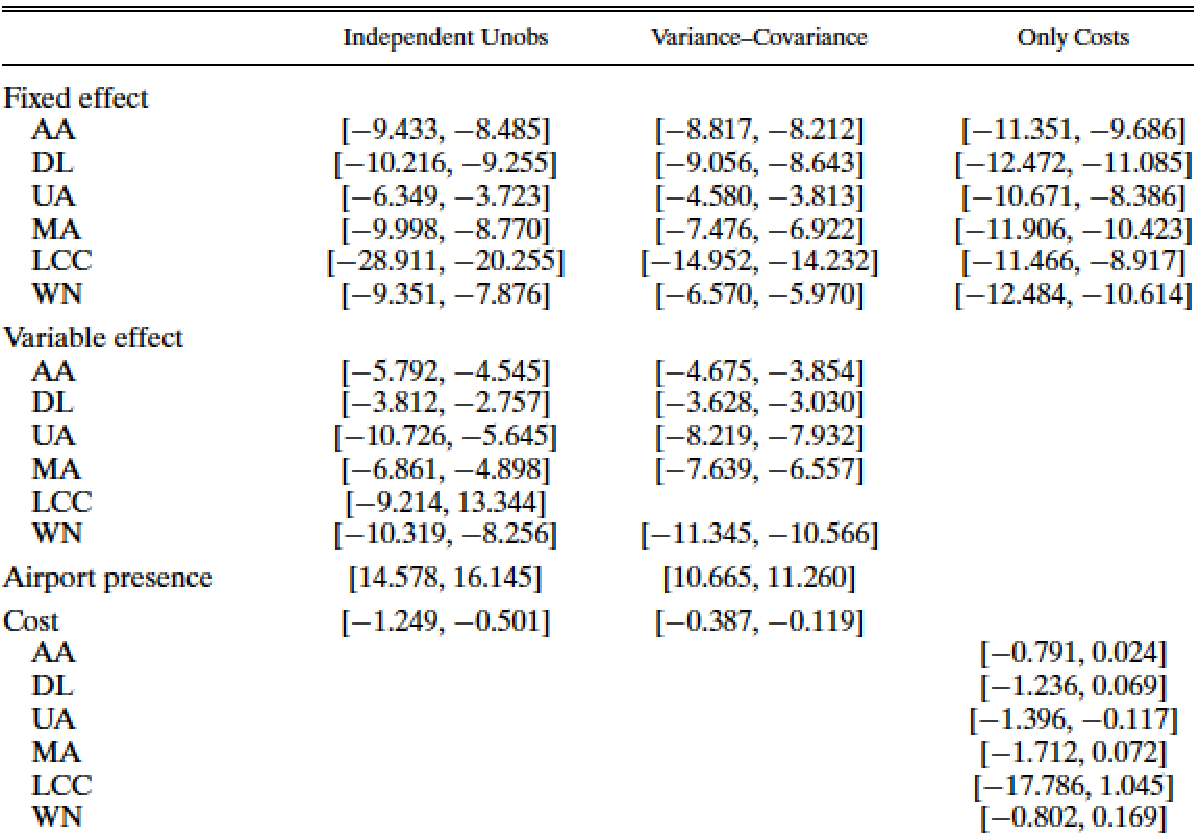
\includegraphics[width=1.0\linewidth]{ciliberto_tamer_table4a.pdf}\\
\end{center}
}

\frame[plain]
{
\frametitle{Results - Ciliberto and Tamer (2009)}
\begin{center}
\tiny
TABLE IV--{\it Continued}\\
\hspace{-.43in}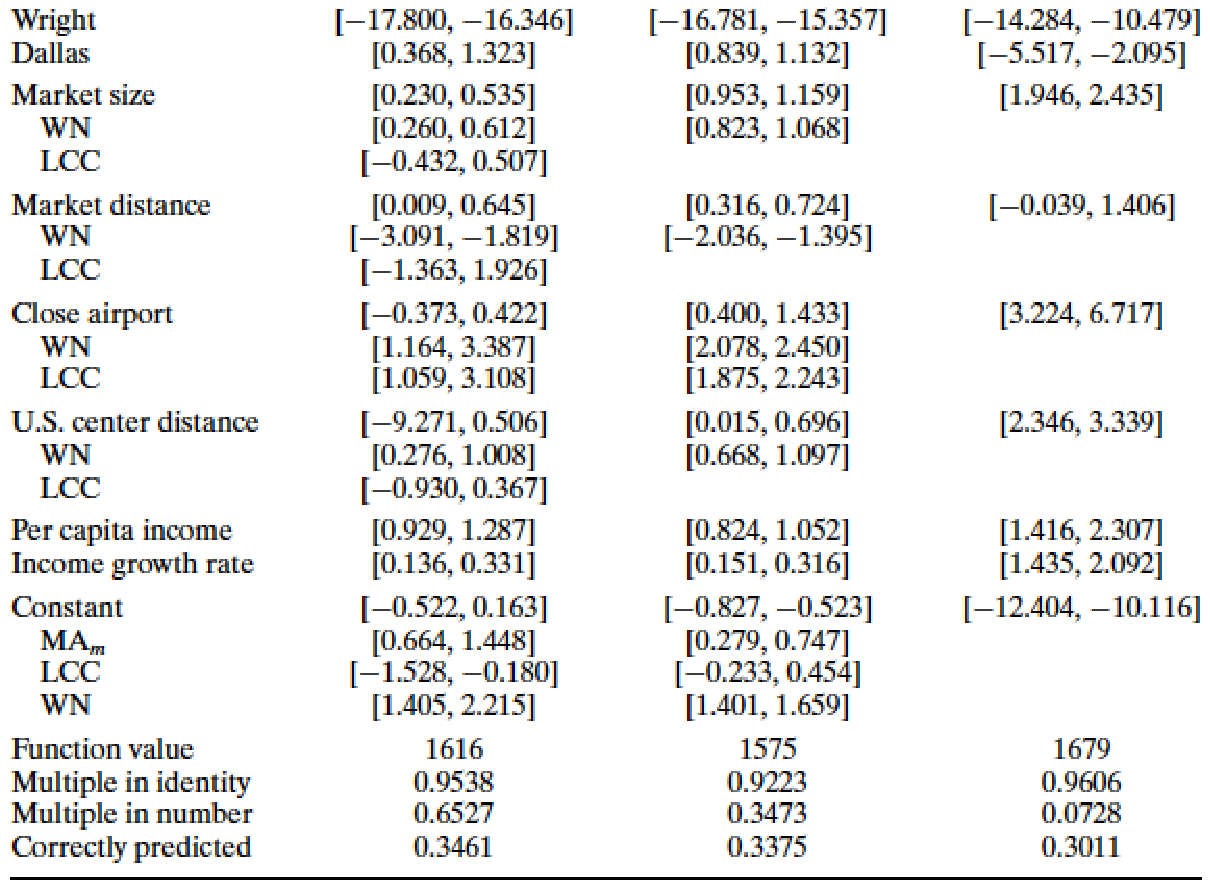
\includegraphics[width=1.0\linewidth]{ciliberto_tamer_table4b.pdf}\\
\end{center}
}

\section{The Profit Inequality Approach}
\frame[plain]
{
\frametitle{The Profit Inequality Approach}
Pakes, Porter, Ho and Ishii\ (2010); Pakes (2010). \\
\vspace{0.2in}
This approach allows for
differences between the primitives that underly agents' decisions and the
econometrician's constructs for those primitives. \\
\vspace{0.2in}
We start with the
measurement model that provides the relationship between these two objects.
}

\frame[plain]
{
\frametitle{The Profit Inequality Approach}
Let our \textit{observable} approximation to $\pi (.)$\\
\begin{equation*}
r^{I}(d,d_{-i},z_{i}^{o},\theta _{0})
\end{equation*}

\vspace{0.2in}
%%%%%%%%%%%Julie - verify that you agree with my classification of this variable as an "error in
%%%%%%%%%%% the approximation" of pi.
Define the error in this approximation as:
\begin{equation*}
\upsilon (d,d_{-i},z_{i}^{o},z_{i},\theta
_{0})=r^{I}(d,d_{-i},z_{i}^{o},\theta _{0})-\pi (d,d_{-i},z_{i}).
\end{equation*}
}

\frame[plain]
{
\frametitle{The Profit Inequality Approach}


Then by definition:%
\begin{equation*}
r^{I}(d,d_{-i},z_{i}^{o},\theta _{0})=\mathit{\varepsilon }\left[ \pi (d_{i},%
\mathbf{d}_{-i},\mathbf{z}_{i})|\mathit{I}_{i}\right] +\upsilon
_{2,i,d}^{I}+\upsilon _{1,i,d}^{I},
\end{equation*}

where%
\begin{equation*}
\upsilon _{2,i,d}^{I}=\mathit{\varepsilon }\left[ \upsilon
(d,d_{-i},z_{i}^{o},z_{i},\theta _{0})|\mathit{I}_{i}\right]
\end{equation*}

and%
\begin{equation*}
\upsilon _{1,i,d}^{I}=\left( \pi (d,.)-\mathit{\varepsilon }\left[ \pi (d,.)|%
\mathit{I}_{i}\right] \right) +\left( \upsilon (d,;)-\mathit{\varepsilon }\left[
\upsilon (d,.)|\mathit{I}_{i}\right] \right) .
\end{equation*}
We will discuss the sources and interpretation of $\upsilon _{1}^{I}$ and $\upsilon _{2}^{I}$ in the following slides.
}

\frame[plain]
{
\frametitle{The Profit Inequality Approach}

Note: For all $d\in D_{i}$, $\mathit{\varepsilon }\left[ \upsilon _{1,i,d}^{I}|%
\mathit{I}_{i}\right] =0$, by construction, while $\mathit{\varepsilon }\left[
\upsilon _{2,i,d}^{I}|\mathit{I}_{i}\right] \neq 0$. It is this distinction
that forces us to keep track of two separate disturbances and consider their
relative importance.\\
\vspace{0.2in}


}

\frame[plain]
{
\frametitle{The Profit Inequality Approach}
\textbf{Sources of $\protect\upsilon _{1}^{I}$:}\\
\vspace{0.2in}
By construction $\upsilon _{1}^{I}$ is the sum of:

\begin{enumerate}
\item Expectational error%
\begin{equation*}
\pi (d,;)-\mathit{\varepsilon }\left[ \pi (d,.)|\mathit{I}_{i}\right]
\end{equation*}%
and

\item Specification and measurement error%
\begin{equation*}
\upsilon (d,;)-\mathit{\varepsilon }\left[ \upsilon (d,.)|\mathit{I}_{i}\right]
\end{equation*}
\end{enumerate}

}

\frame[plain]
{
\frametitle{The Profit Inequality Approach}

The expectational error is caused by:
\begin{enumerate}[i]
\item uncertainty in $\mathbf{z}_{i}$,
and/or 
\item asymmetric information which is uncertainty in $\mathbf{d}_{-i}$%. 
\end{enumerate}
\vspace{0.1in}

So to compute its distribution (as we'd need to if we were using MLE, for
example), we'd have to specify what each agent knew about its competitors,
and then repeatedly solve for an equilibrium (a process which would
typically require us to select among equilibria). \\
\vspace{0.2in}
Since we'd have to compute
returns from a counterfactual, the specification error would probably be
non-trivial. The inequalities methodology does not require this step.

}

\frame[plain]
{
\frametitle{The Profit Inequality Approach}
\textbf{Sources of $\protect\upsilon _{2}^{I}$ and Selection:}\\
\vspace{0.2in}
$\upsilon _{2}^{I}$ is that part of profits that the agent does condition on
when making its decision but the econometrician has not included in the
profit specification. \\
\vspace{0.2in}
Since $\upsilon _{2,i}^{I}\in \mathit{I}_{i}$ and $%
d_{i}=d(\mathit{I}_{i})$, $d_{i}$ will generally be a function of $\upsilon
_{2,i}^{I}$ (and perhaps also of $\upsilon _{2,-i}^{I}$).  \\
\vspace{0.2in}
This can generate a selection problem.

}

\frame[plain]
{
\frametitle{The Profit Inequality Approach}

For example, temporarily ignore any difference between the agent's expectations (our 
$\mathit{\varepsilon }(.)$) and the expectations generated by the true data
generating process (our $E(.)$). \\
\vspace{0.2in}
Assume that $x$ is an ``instrument" in the
sense that $\mathit{\varepsilon }(\upsilon _{2}^{I}|x)=0$, and, in addition,
that $x\in I$. Then:%
\begin{equation*}
\mathit{\varepsilon }(\upsilon _{1}^{I}|x)=\mathit{\varepsilon }(\upsilon
_{2}^{I}|x)=0.
\end{equation*}


}

\frame[plain]
{
\frametitle{The Profit Inequality Approach}
However, these expectations do not condition on $d_{i}$\\
\vspace{0.2in}
Any moment
which depends on $d_{i}$ (ie on the choice made by agent $i$ - all our
inequalities depend on this) requires properties of the disturbance
conditional on $d_{i}$. \\
\vspace{0.2in}
Since $d$ is measurable given the information set $%
\mathit{I}$, 
\begin{equation*}
\mathit{\varepsilon }(\upsilon _{1}^{I}|x,d)=0.
\end{equation*}
}

\frame[plain]
{
\frametitle{The Profit Inequality Approach}


However, since $\upsilon _{2}\in \mathit{I}$, and 
\begin{equation*}
\mathit{\varepsilon }(\pi (.)|.)=\mathit{\varepsilon }(r(.)|.)-\upsilon _{2},
\end{equation*}

if the agent chooses $d^{\ast }$ then 
\begin{equation*}
\upsilon _{2,d}-\upsilon _{2,d^{\ast }}\geq \mathit{\varepsilon }(r(.,d)|.)-%
\mathit{\varepsilon }(r(.,d^{\ast })|.)
\end{equation*}

so%
\begin{equation*}
\boxed{\mathit{\varepsilon }(\upsilon _{2,d}|x,d)\neq 0.}
\end{equation*}
More intuitively: firms are choosing $d^{\ast }$ based on the observed $%
v_{2,d^{\ast }}$, so it makes sense that there's a selection issue, ie that $%
\mathit{\varepsilon }(\upsilon _{2,d^{\ast }}|x,d^{\ast })\neq 0.$

}

\frame[plain]
{
\frametitle{The Profit Inequality Approach}
This result
implies that the statement that ``$x$ is an instrument"\ does not ``solve" the
selection problem. Formally%
\begin{equation*}
\mathit{\varepsilon }\left[ \Delta \pi (d_{i},.)|x_{i},d_{i}\right] =\mathit{%
\varepsilon }\left[ \Delta r(d_{i},.)|x_{i},d_{i}\right] -\mathit{\varepsilon }%
\left[ \upsilon _{2,i,d_{i}}^{I}-\upsilon _{2,i,d^{\prime }}^{I}|x_{i},d_{i}%
\right] .
\end{equation*}

Theory gives us $\mathit{\varepsilon }\left[ \Delta \pi (d_{i},.)|x_{i},d_{i}%
\right] \geq 0$, but this only implies 
\begin{equation*}
\mathit{\varepsilon }\left[ \Delta r(d_{i},.)|x_{i},d_{i}\right] \geq 0
\end{equation*}

if 
\begin{equation*}
\mathit{\varepsilon }\left[ \upsilon _{2,i,d_{i}}^{I}-\upsilon _{2,i,d^{\prime
}}^{I}|x_{i},d_{i}\right] \geq 0,
\end{equation*}

and \textit{this requires additional conditions on the measurement model. }We will come back to these conditions
shortly.\\ (See IC4.)
}
\section{The Additional Requirements for Profit Inequalities}

\frame[plain]
{
\frametitle{The Additional Requirements for Profit Inequalities}
Recall that we need an assumption on the relationship between agents'
expectations and the expectation operator generated by the data generating
process, plus restrictions on the measurement model.
\vspace{0.1in}
\begin{enumerate}
\setcounter{enumi}{2}
  \item \textbf{Agents' Expectations (IC3)}

Let $h(.)$ be a positive valued function. There is a known subset of the
observed variables, say $x_{i}\in \mathit{I}_{i}$, that satisfy:%
\begin{equation*}
\frac{1}{N}\sum_{i}\mathit{\varepsilon }\left[ \Delta \pi (d_{i},d^{\prime
},d_{-i},z_{i})|x_{i}\right] \geq 0\Rightarrow
\end{equation*}%
\begin{equation*}
E\left[ \frac{1}{N}\sum_{i}\left[ \Delta \pi (d_{i},d^{\prime
},d_{-i},z_{i})h(x_{i})\right] \right] \geq 0.
\end{equation*}
\end{enumerate}

}

\frame[plain]
{
\frametitle{The Additional Requirements for Profit Inequalities}
\textbf{Correct Expectations are Sufficient.}
\vspace{0.2in}
\begin{itemize}
\item Standard condition - each agent knows:
\begin{enumerate}[i]
\item the other agents' strategies ($\mathbf{d}_{-i}(\mathit{I}_{-i})$), and 
\item the joint distribution of other agents' information sets and the primitive sources of
uncertainty (of $(\mathit{I}_{-i},\mathbf{z}_{-i})$) conditional on $\mathit{%
I}_{i}$, and regularity conditions.
\end{enumerate}
\vspace{0.2in}
\item Weaker condition:\ agents' conditional expectations of the profit
difference are correct. 
\begin{itemize} \item This does not require knowledge of other agents'
strategies, or the distribution of $(\mathbf{d}_{-i},\mathbf{z}_{i})$
conditional on $\mathit{I}_{i}$. 
\item Agent uncertainty is permitted and
we do not need to fully specify how the agent forms its expectations.
\end{itemize}
\end{itemize}

}

\frame[plain]
{
\frametitle{The Additional Requirements for Profit Inequalities}
\textbf{Incorrect Expectations are Possible.}\\
\vspace{0.2in}
All we need is the average of 
\begin{equation*}
\mathit{\varepsilon }\left[ \Delta \pi (d_{i},d^{\prime },d_{-i},z_{i})|x_{i}%
\right] -E\left[ \Delta \pi (d_{i},d^{\prime },d_{-i},z_{i})|x_{i}\right]\geq 0
\end{equation*}%
Relevant cases:

\begin{itemize}
\item Agents' beliefs are not exactly right but the difference between
agents' expectations on $\Delta \pi (.,\theta _{0})$ and the expectation of
the data generating process are mean-zero conditional on $x$ (in that case
the expression is satisfied with equality). Or

\item Agents can be ``consistently overly optimistic" about the relative
profits from the decisions they make.
\end{itemize}


}

\frame[plain]
{
\frametitle{The Additional Requirements for Profit Inequalities}
\begin{enumerate}
\setcounter{enumi}{3}
  \item \textbf{Condition on the Measurement Model (IC4)}
This final condition is designed to deal with the selection problem noted
above. Assume $D_{i}$ is discrete. $\exists $ observed $x\in \mathit{I}_{i}$
and a function $c(.):D_{i}$ $\times $ $D_{i}\rightarrow R^{+}$ such that we
satisfy:%
\begin{equation*}
E\left[ \sum_{j\in D_{i}}\chi \left\{ d_{i}=j\right\} c(j,d^{\prime
}(j))\left( \upsilon _{2,i,j}^{I}-\upsilon _{2,i,d^{\prime }(j)}^{I}\right)
h(x_{i})\right] \geq 0
\end{equation*}%
where $\chi \left\{ d_{i}=j\right\} $ is an indicator function.
\end{enumerate}
}

\frame[plain]
{
\frametitle{The Additional Requirements for Profit Inequalities}
\textbf{Notes regarding IC4}\\
\vspace{0.2in}
\begin{itemize}
\item This expectation is an unconditional average (does not condition on $d_{i}$); for
every possible $d\in D_{i}$ we specify a $d^{\prime }(d)$.
\vspace{0.1in}
\item This average is an average in the \textit{differences} in the $%
\upsilon _{2,i,j}^{I}-\upsilon _{2,i,d^{\prime }(j)}^{I}$.
\vspace{0.1in}
\item Both (i) the weights and (ii) the comparison ($d^{\prime }$) can vary
with $j$.
\end{itemize}

}

\frame[plain]
{
\frametitle{The Additional Requirements for Profit Inequalities}
\textbf{Satisfying IC4}\\
\begin{itemize}
\item $\forall d,\upsilon _{2,i,d}=\upsilon _{2,i}$. 
\begin{itemize}
\item This is Hansen and
Singleton's (1982)\ classic article, but can allow for discreteness in
choice sets, choices which are on the boundaries of the choice set, and
interacting agents.
\end{itemize}
\end{itemize}

}

\frame[plain]
{
\frametitle{The Additional Requirements for Profit Inequalities}
\textbf{Satisfying IC4 (continued)}\\
\begin{itemize}
\item $\upsilon _{2,i,d}$ can vary across decisions, but the same value of $%
\upsilon _{2,i,d}^{I}$ appears in more than one of them (so there are
``group" effects).
\begin{itemize}
\item Examples:\begin{itemize} \item Entry models with location-specific fixed effects, \item Social
interaction models with group effects, \item Panel data discrete choice models
with choice-specific fixed effects, and \item Cross-sectional discrete choice
models where the same $\upsilon _{2,i,d}^{I}$ appear in more than one
choice. \end{itemize}
\item For each choice $d_{i}=j$,
pick an alternative $d^{\prime }(d)$ such that the two choices have the same
value of $\upsilon _{2,i,d}$\begin{itemize} \item e.g. pick an alternative in the same market;
the same group; a firm making the same choice in a different time period.
\end{itemize}
\item The $\upsilon _{2}$ terms will difference out when we generate the
inequality.
\end{itemize}
\end{itemize}

}

\frame[plain]
{
\frametitle{The Additional Requirements for Profit Inequalities}
\textbf{Satisfying IC4 (continued)}\\
\begin{itemize}
\item Ordered choice models (including the vertically-differentiated demand
model used in I.O.). 
\begin{itemize} \item E.g. the firm is buying a discrete number of units, so $%
d_{i}\in Z_{+}$ and $\upsilon _{2,i}$ is a cost component known to the agent
but not the econometrician. \item Take $d^{\prime }(j)=j+1$. The difference in
profits will always contain $\upsilon _{2}$, now interpreted as the cost
savings from not purchasing the additional unit. \item We will take an
unconditional average across this cost (not conditional on the choice). \item This
is the method used in Ishii\ (2005).
\end{itemize}
\end{itemize}

}

\frame[plain]
{
\frametitle{The Additional Requirements for Profit Inequalities}
\textbf{Satisfying IC4 (continued)}\\
\begin{itemize}
\item Contracting models in which $\upsilon _{2}$ is interpreted as a
component of the contract that the agents know but the econometrician does
not. 
\begin{itemize} 
\item The cost is a profit to the seller if the contract is established
and a saving to the buyer if the contract is not accepted. 
\item We can difference
it out by adding together the inequality of the buyer and that of the
seller. 
\item This is an extension of the model in Ho\ (2009); the original paper
takes account of $\upsilon _{1}$ but ignores $\upsilon _{2}$.
\end{itemize}

\end{itemize}

}

\frame[plain]
{
\frametitle{The Additional Requirements for Profit Inequalities}
\textbf{Satisfying IC4 (continued)}\\
\begin{itemize}
\item Models for micro data where a variable needed for an inequality is
unobserved (or is measured with error)\ at the micro level but is observed
at a higher level of aggregation (say because of the availability of Census
data).
\end{itemize}
}

\section{Estimation from Profit Inequalities}
\frame[plain]
{
\small
C1 and C2 imply that for each $i$%
\begin{equation*}
0\leq \sum_{j}\mathit{\varepsilon }\left( \chi \left\{ d_{i}=j\right\}
c(j,d^{\prime }(j))\Delta \pi (j,d^{\prime }(j),.)\right) h(x_{i}).
\end{equation*}

Average over $i$. IC3 implies that this average is less than or equal to%
\begin{equation*}
E\left[ \frac{1}{N}\sum_{i}\sum_{j}\left( \chi \left\{ d_{i}=j\right\}
c(j,d^{\prime }(j))\Delta \pi (j,d^{\prime }(j),.)\right) h(x_{i})\right] ,
\end{equation*}

which from IC4 is less than%
\begin{equation*}
E\left[ \frac{1}{N}\sum_{i}\sum_{j}\left( \chi \left\{ d_{i}=j\right\}
c(j,d^{\prime }(j))\Delta r(j,d^{\prime }(j),.)\right) h(x_{i})\right] .
\end{equation*}

Since this last inequality is in terms of \textit{observable} moments, we
can use its sample analogue as a basis for estimation.

\frametitle{Estimation from Profit Inequalities}
}

\frame[plain]
{
\frametitle{Estimation from Profit Inequalities - Katz (2007)}
Katz's problem was to estimate the costs shoppers assign to driving to a
supermarket. \\
\vspace{0.2in}
These costs are important for the choice of supermarket
locations and, as a result, for the analysis of the impact of zoning
regulations. \\
\vspace{0.2in}
They have been difficult to analyze empirically with standard
choice models because of the complexity of the choice set facing consumers
(all possible bundles of goods at all supermarkets).
}

\frame[plain]
{
\frametitle{Estimation from Profit Inequalities - Katz (2007)}
Assume that the agents' utility functions are additively separable functions
of:\begin{itemize} \item the utility from the basket of goods the agent buys, \item expenditure on that basket, and \item drive time to the supermarket. \end{itemize}
\vspace{0.1in}
Since utilities are only defined up to a monotone transformation, there is a free normalization for each individual. Katz normalizes the coefficient on expenditure for each individual to equal one. \\
\vspace{0.2in}
He allows for heterogeneity in the cost of
drive time that is known to the agents when they make their decision but
unobserved by the econometrician.  This will be one component of $\upsilon
_{2,i}$.
}

\frame[plain]
{
\frametitle{Estimation from Profit Inequalities - Katz (2007)}
Possible counterfactuals:
Purchase of any bundle of goods at any store. \\
\vspace{0.2in}
For a particular $d_{i}$ choose $d^{\prime }(d_{i})$ to be the purchase of
\begin{itemize}
\item the same basket of goods

\item at a store which is further away from the consumer's home than the
store the consumer shopped at.
\end{itemize}
}

\frame[plain]
{
\frametitle{Estimation from Profit Inequalities - Katz (2007)}
This choice of $d^{\prime }(d_{i})$ allows us to difference out the impact
of the basket of goods chosen on utility. \\
\vspace{0.2in}
I.e. if $e(d)$ and $dt(d)$ provide
the expenditure and the drive time for store choice $d$, and $(\theta
+\upsilon _{2,i})$ is agent $i$'s cost of drive time (in units of
expenditure),%
\small
\begin{equation*}
\mathit{\varepsilon }\left[ \sum_{j}\chi \left\{ d_{i}=j\right\} \Delta \pi
(j,d^{\prime }(j),z_{i})|I_{i}\right] =
\end{equation*}%
\begin{equation*}
\mathit{\varepsilon }\left[ \sum_{j}\chi \left\{ d_{i}=j\right\} \left(
e(j)-e(d^{\prime }(j))+(\theta +\upsilon _{2,i})\left( dt(j)-dt(d^{\prime
}(j))\right) \right) |I_{i}\right] \geq 0,
\end{equation*}
\begin{equation*}
\text{ at }\theta =\theta _{0}.
\end{equation*}

}

\frame[plain]
{
\frametitle{Estimation from Profit Inequalities - Katz (2007)}
Assuming, as seems reasonable, that $(dt\left( d_{i}),dt\left( d^{\prime
}(d_{i})\right) \right) \subset I_{i}$, this together with the fact that $%
dt(j)-dt(d^{\prime }(j))<0$ by choice of alternative implies that:%
\begin{equation*}
\mathit{\varepsilon }\left[ \sum_{j}\chi \left\{ d_{i}=j\right\} \left( \frac{%
e(j)-e(d^{\prime }(j))}{dt(d^{\prime }(j))-dt(j)}-(\theta +\upsilon
_{2,i})\right) |I_{i}\right] \leq 0.
\end{equation*}
}

\frame[plain]
{
\frametitle{Estimation from Profit Inequalities - Katz (2007)}
Let $\theta $ be the average of the cost of drive time across consumers, so $%
\sum_{i}\upsilon _{2,i}=0$ by construction, and assume IC3. Then:%
\begin{equation*}
E\left[ \frac{1}{N}\sum_{i}\left( \frac{e(d_{i})-e(d^{\prime }(d_{i}))}{%
dt(d^{\prime }(d_{i}))-dt(d_{i})}\right) \right] -\theta \leq 0,\text{ }at%
\text{ }\theta =\theta _{0}.
\end{equation*}

}

\frame[plain]
{
\frametitle{Estimation from Profit Inequalities - Katz (2007)}
This result provides a lower bound to $\theta $. \\
\vspace{0.2in}
Were we to consider a second
alternative in which the bundle of goods purchased was the same as in the
actual choice but the counterfactual store required \textit{less drive time}%
, we would also get an upper bound to $\theta _{0}$. \\
\vspace{0.2in}
Katz (2007) shows that
these bounds are quite informative and provides a range for the average cost
of drive time which accords with auxiliary information, while more standard
discrete choice estimators do not.

}

\frame[plain]
{
\frametitle{Estimation from Profit Inequalities - Katz (2007)}
To obtain these inequalities we chose an alternative that allowed us to
difference out the impact of the bundle of goods chosen on utility
(differencing out our "group" effect).\\
\vspace{0.2in}
We then rearranged these differences
to form a moment which was linear in the remaining source of $\upsilon _{2}$
variance no matter $d_{i}$ (the source being differences in the costs of
travel time). }

\frame[plain]
{
\frametitle{Estimation from Profit Inequalities - Katz (2007)}
If we were interested in the impact of a particular good
purchased on utility, we would have considered baskets of goods which
differed only in that good and goods which had cross partials with that good
in the utility function, at the \textit{same} supermarket (thus differencing
out the effects of travel time and other components of utility). \\
\vspace{0.2in}A lot more
options would present themselves were we to have data on multiple shopping
trips for each household.

}
\section{Summary}
\frame[plain]
{
\frametitle{Summary}
\textbf{Full Information - No Error Model}\\
\begin{itemize}
\item Does not allow for:

\begin{itemize}
\item Specification or measurement error

\item Asymmetric or incomplete information

\item Incorrect expectations
\end{itemize}

except to the extent that these details do not cause differences in the
profits earned from different choices.
\vspace{0.1in}
\item Requires a parametric assumption on the distribution of $\upsilon
_{2}$.

\end{itemize}

}
\frame[plain]
{
\frametitle{Summary}
\textbf{Profit Inequalities Model}

\begin{itemize}
\item Allows for specification errors, incorrect expectations, and
incomplete and asymmetric information.
\vspace{0.1in}
\item The econometrician does not need to specify what the agent knows about
either its competitors, or about the state of nature.
\vspace{0.1in}
\item However, it requires a (sometimes tricky) restriction on $\upsilon
_{2} $. 
\begin{itemize} \item Given that restriction, there is no need for a
distributional assumption here.
\end{itemize}
\end{itemize}


}

\end{document}